\documentclass[a4]{beamer}
\usepackage{amssymb}
\usepackage{graphicx}
\usepackage{subfigure}
\usepackage{newlfont}
\usepackage{amsmath,amsthm,amsfonts}
%\usepackage{beamerthemesplit}
\usepackage{pgf,pgfarrows,pgfnodes,pgfautomata,pgfheaps,pgfshade}
\usepackage{mathptmx}  % Font Family
\usepackage{helvet}   % Font Family
\usepackage{color}

\mode<presentation> {
 \usetheme{Default} % was Frankfurt
 \useinnertheme{rounded}
 \useoutertheme{infolines}
 \usefonttheme{serif}
 %\usecolortheme{wolverine}
% \usecolortheme{rose}
\usefonttheme{structurebold}
}

\setbeamercovered{dynamic}

\title[MA4413]{Statistics for Computing \\ {\normalsize Lecture 2B}}
\author[Kevin O'Brien]{Kevin O'Brien \\ {\scriptsize Kevin.obrien@ul.ie}}
\date{Autumn Semester 2013}
\institute[Maths \& Stats]{Dept. of Mathematics \& Statistics, \\ University \textit{of} Limerick}

\renewcommand{\arraystretch}{1.5}

\begin{document}

\begin{frame}
\titlepage
\end{frame}

\frame{

\frametitle{This Class}
\begin{itemize}
\item SULIS
\item Midterm in Week 5
\item Teaching: Discrete Random Variables
\item Teaching: Graphical Methods (Principally Histograms)
\end{itemize}
}



\frame{

\frametitle{Graphical Procedures for Statistics}
\begin{itemize}
\item Bar-plots
\item Histograms
\item Boxplots

\end{itemize}
}
%----------------------------------------------------------------%
\frame{
\frametitle{Histograms}
\begin{itemize}
\item Consider an experiment in which each student in a class of 60 rolls a die 100 times.
\item Each score is recorded, and a total score is calculated.
\item As the expected value of rolled die is 3.5, the expected total is 350 for each student.
\item At the end of the experiment the students reported their totals.
\item The totals were put into ascending order, and tabulated as follows (next slide).
\end{itemize}

}

%--------------------------------------------------------%
\frame{
\frametitle{Outcomes of die-throw experiment}
\small
\begin{center}
\begin{tabular}{|c c c c c c c c c c|}
  \hline
  % after \\: \hline or \cline{col1-col2} \cline{col3-col4} ...
307 & 321 & 324 & 328 & 329 & 330 & 334 & 335 & 336 &337 \\
337 & 337 & 338 & 339 & 339 & 342 & 343 & 343 & 344 &344 \\
346 & 346 & 347 & 348 & 348 & 348 & 350 & 351 & 352 &352 \\
353 & 353 & 353 & 354 & 354 & 356 & 356 & 357 & 357 &358 \\
358 & 360 & 360 & 361 & 362 & 363 & 365 & 365 & 369 &369 \\
370 & 370 & 374 & 378 & 381 & 384 & 385 & 386 & 392 &398 \\
  \hline
\end{tabular}
\end{center}
\normalsize
\begin{itemize}
\item What proportion of outcomes are less than or equal to 330? \\ (Answer: $10\%$)
\item What proportion of outcomes are greater than or equal to 370?\\ (Answer: $16.66\%$)
\end{itemize}
}
%--------------------------------------------------------%

\frame{
\frametitle{What is a Histograms}



}
%--------------------------------------------------------%

\frame{
\frametitle{Histograms}
For the die-throw experiment;
\begin{center}
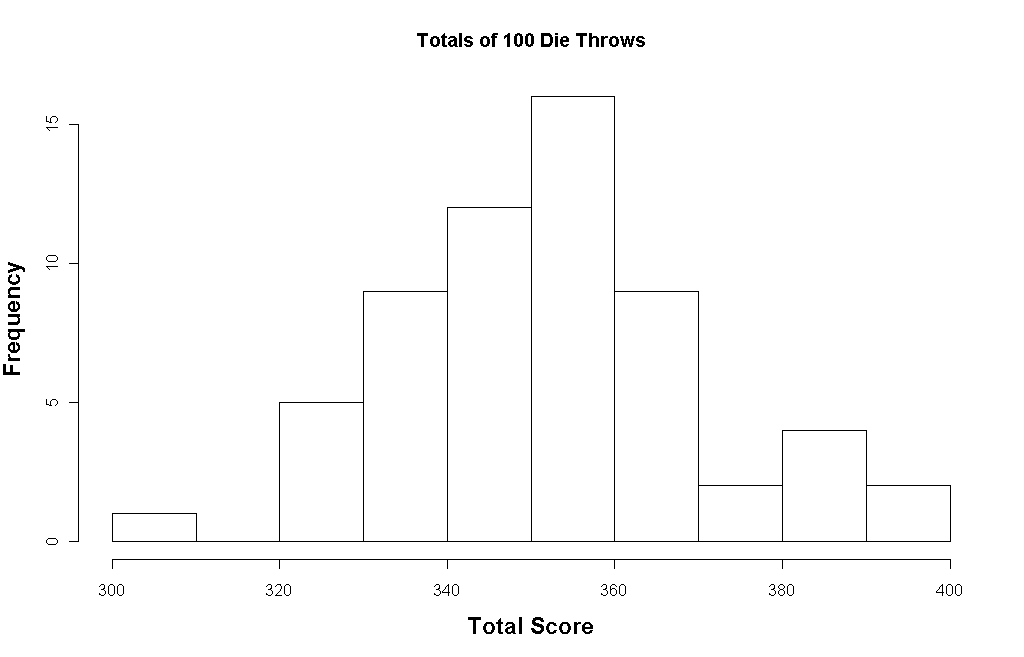
\includegraphics[scale=0.30]{3aDieHist}
\end{center}

}
%----------------------------------------------------------------%
\frame{
\frametitle{Constructing Histograms}
\begin{itemize}
\item Compute an appropriate number of class intervals.
\item As a rule of thumb, the number of class intervals is usually approximately the square root of the number of observations.
\item As there are 60 observations, we would normally use 7 or 8 class intervals.
\item To save time, we will just use 5 class intervals.
\end{itemize}

}
%----------------------------------------------------------------%
\frame{
\frametitle{Frequency Tables}


}
%--------------------------------------------------------%

\frame{
\frametitle{Histograms}

\begin{center}
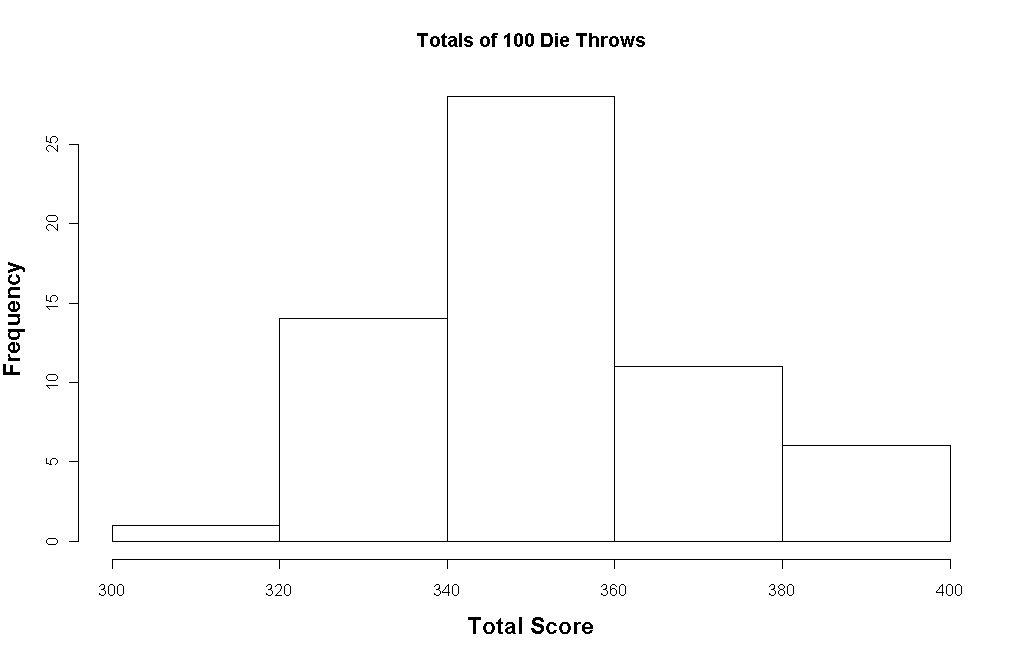
\includegraphics[scale=0.30]{3aDieHist2}
\end{center}

}
%--------------------------------------------------------%

\frame{
\frametitle{Histograms}
\begin{itemize}
\item Suppose that the experiment of throwing a die 100 times and recording the total was repeated 100,000 times.
\item (If implemented on a computer, we would call this a simulation study)
\item The histogram of data (with a class interval width of 2) is shown on the next slide.
\item How should the shape of the histogram be described?
\item ``Bell-shaped" would be a suitable description.
\end{itemize}
}
%--------------------------------------------------------%

\frame{
\frametitle{Histograms}

\begin{center}
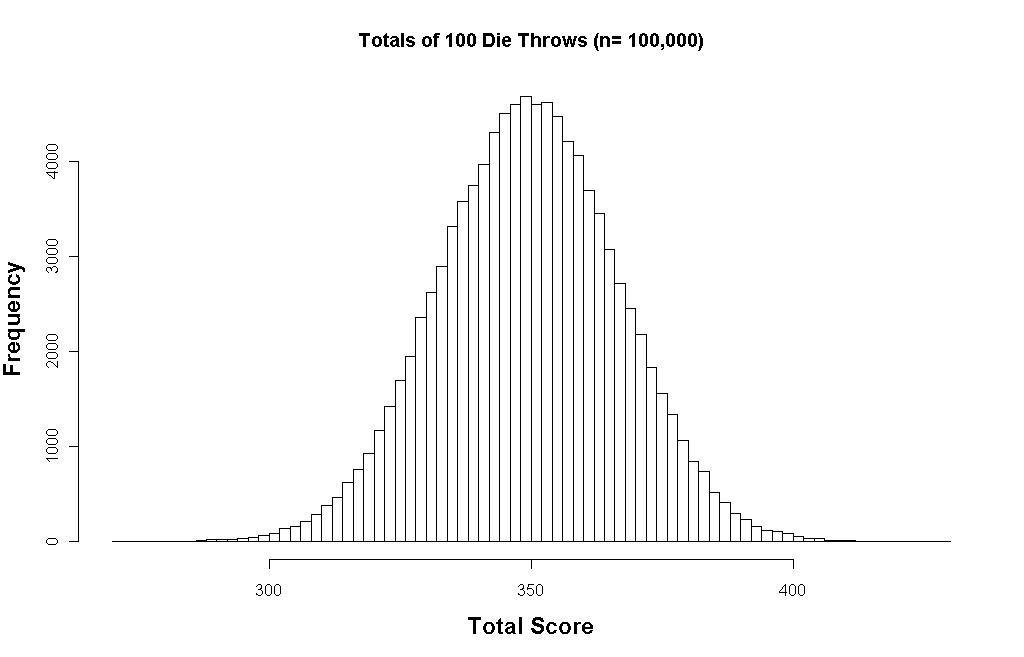
\includegraphics[scale=0.30]{3aDieHist3}
\end{center}

}
%--------------------------------------------------------%

\frame{
\frametitle{Simulation Study}
A couple of remarks about the simulation study, some of which will be relevant later on.
\begin{itemize}
% \item Approximately 76\% of the values are between 330 and 370.
\item Approximately 68.7\% of the values in the simulation study are between 332 and 367.
\item Approximately 95\% of the values are between 316 and 383.
\item $2.5\%$ of the values output are less than 316.
\item $2.5\%$ of the values study output are greater than 383.
\item 175 values are greater than or equal to 400, whereas 198 values are less than or equal to 300.
\item Results such as these are unusual, but they are not impossible.
\end{itemize}
}

%--------------------------------------------------------%

\frame{
\frametitle{Random Variables}
A pair of dice is thrown. Let X denote the minimum of the two numbers which occur.
Find the distributions and expected value of X.
}
%-------------------------------------------------------------%
\frame{
\frametitle{Random Variables}
A fair coin is tossed four times.
Let X denote the longest string of heads.
Find the distribution and expectation of X.}
%-------------------------------------------------------------%
\frame{\frametitle{Random Variables}
A fair coin is tossed until a head or five tails occurs.
Find the expected number E of tosses of the coin.}
%-------------------------------------------------------------%
\frame{\frametitle{Random Variables}A coin is weighted so that P(H) = 0.75 and P(T ) = 0.25

The coin is tossed three times. Let X denote the number of
heads that appear.
\begin{itemize}
\item (a) Find the distribution f of X.
\item (b) Find the expectation E(X).
\end{itemize}
}

%-------------------------------------------------------------%
\frame{
\begin{itemize}
\item Now consider an experiment with only two outcomes. Independent repeated trials of such an experiment are
called Bernoulli trials, named after the Swiss mathematician Jacob Bernoulli (1654�1705). \item The term \textbf{\emph{independent
trials}} means that the outcome of any trial does not depend on the previous outcomes (such as tossing a coin).
\item We will call one of the outcomes the ``success" and the other outcome the ``failure".
\end{itemize}
}

%-------------------------------------------------------------%
\frame{
\begin{itemize} \item
Let $p$ denote the probability of success in a Bernoulli trial, and so $q = 1 - p$ is the probability of failure.
A binomial experiment consists of a fixed number of Bernoulli trials. \item A binomial experiment with $n$ trials and
probability $p$ of success will be denoted by
\[B(n, p)\]
\end{itemize}
}
%-------------------------------------------------------------%


\end{document}



%---------------------------------------------------------------------------------------------------------------%
%----R Code ----
%---------------------------------------------------------------------------------------------------------------%
n=60000
Y=numeric(n)
for ( i in 1:n){

X=floor(runif(100,1,7))
Y[i]=sum(X)
}

Y
hist(Y,breaks=seq(300,400,by=10),main=c("Totals of 100 Die Throws"),cex.lab=1.4,font.lab=2,xlab=c("Total Score"))

hist(Y,breaks=seq(300,400,by=20),main=c("Totals of 100 Die Throws"),cex.lab=1.4,font.lab=2,xlab=c("Total Score"))



Z=seq(1:n)
Y/Z

plot(Y/Z,type="l",col="red",main=c("Die Rolls: Running Average"),font.lab=2,ylab="Average Value", xlab=
" Number of Throws")
abline(h=3.5,col="green")


#####################################################

plot(Z,Z.y,pch=16,col="red",ylim=c(2.5,5.5),main=c("Variance"),font.lab=2,ylab=" ", xlab="X: Green  Y: Blue  Z: Red" )

points(Y,Y.y,pch=16,col="blue" )
points(X,X.y,pch=16,col="green" )
points(c(1000,1000,1000),c(3,4,5),pch=18,cex=1.2)
lines(c(1000,1000),c(2.75,5.25),lty=3)



n=100000
Y=numeric(n)
for ( i in 1:n){

X=floor(runif(100,1,7))
Y[i]=sum(X)
}

Y
hist(Y,breaks=seq(270,430,by=2),main=c("Totals of 100 Die Throws (n= 100,000)"),cex.lab=1.4,font.lab=2,xlab=c("Total Score")) 